
\documentclass[]{scrartcl}

% Use utf-8 encoding for foreign characters
\usepackage[utf8]{inputenc}

% Setup for fullpage use
\usepackage{fullpage}

% Mathematical symbols
\usepackage{amssymb}

\usepackage[usenames]{color} 

% Uncomment some of the following if you use the features
%
% Running Headers and footers
%\usepackage{fancyhdr}

% Multipart figures
\usepackage{subfigure}

% More symbols
\usepackage{amsmath}
\usepackage{amssymb}
\usepackage{amsthm}
%\usepackage{latexsym}

% We want publication-ready tables.
\usepackage{booktabs}
\usepackage{multirow}

% Surround parts of graphics with box
\usepackage{boxedminipage}

% Package for including code in the document
\usepackage{listings}

% If you want to generate a toc for each chapter (use with book)
\usepackage{minitoc}

% This is now the recommended way for checking for PDFLaTeX:
\usepackage{ifpdf}

% custom float for source listings
\usepackage{float}
\floatstyle{ruled}
\newfloat{program}{htb}{lop}
\floatname{program}{Listing}

%\newif\ifpdf
%\ifx\pdfoutput\undefined
%\pdffalse % we are not running PDFLaTeX
%\else
%\pdfoutput=1 % we are running PDFLaTeX
%\pdftrue
%\fi

\ifpdf
\usepackage[pdftex]{graphicx}
\else
\usepackage{graphicx}
\fi

\usepackage[ruled,vlined,linesnumbered]{algorithm2e}


\usepackage{hyperref}


\ifpdf
\DeclareGraphicsExtensions{.pdf, .jpg, .tif}
\else
\DeclareGraphicsExtensions{.eps, .jpg}
\fi




 
%%% BEGIN DOCUMENT
\begin{document}

\title{Datenhaltung - Sommersemester 2008}

\author{}



\maketitle
\tableofcontents

\section{Relationale Algebra}

\subsection{Join}

\paragraph{allgemeiner Verbund.} F\"ur zwei Relationen $R$ und $S$ und eine Selektionsbedingung $c$ ist der allgemeine Verbund definiert als
$$ R \bowtie_{c} S := \{ r \cup s : r \in R \wedge s \in S \wedge c \} $$
Das ist \"aquivalent zu 
$$ \sigma_{c} (R \times S)$$

\paragraph{Equijoin. } In diesem Speziallfall bestimmt die Selektionsbedingung die Gleichheit eines Attributes $A$ von $R$ und eines Attributes $B$ von $S$.
$$R \bowtie_{A = B} S := \{ r \cup s : r \in R \wedge s \in S \wedge r_{[A]} = s_{[B]} \}$$
Das ist \"aquivalent zu 
$$ \sigma_{[A = B]} (R \times S)$$

\paragraph{Natural Join.} Ein Natural Join setzt sich zusammen aus einem Equijoin und dem Ausblenden gleicher Spalten. F\"ur zwei Relationen $R(A_{1},\dots, A_{n},B_{1},\dots,B_{n})$ und $S(B_{1},\dots,B_{n},C_{1},\dots,C_{n})$ ist
$$R \bowtie S := \{ r \cup s_{[C_{1}, \dots, C_{n}]} : r \in R \wedge s \in S \wedge r_{[B_{1, \dots, B_{n}}]} = s_{[B_{1, \dots, B_{n}}]} \}$$



\section{\underline{E}ntity \underline{R}elationship \underline{M}odel }

\subsection{Kardinalit\"aten}

\paragraph{Teilnehmerkardinalit\"aten.}
\begin{itemize}
\item $E1$ steht in Relation zu 0 oder 1 $E2$
\item $E2$ steht in Relation zu 1 bis $n$ $E1$
\end{itemize}


\begin{figure}[htbp]
\begin{center}
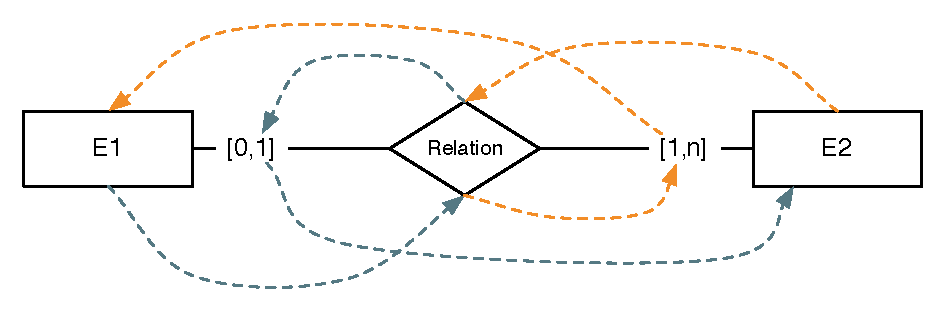
\includegraphics[scale=0.7]{figures/Teilnehmerkardinalitaet.pdf}
\caption{Leserichtung f\"ur Teilnehmerkardinalit\"aten}
\label{default}
\end{center}
\end{figure}




\section{Relationaler Entwurf}

\paragraph{Mehrwertige Abh\"angigkeit (Multi-Valued Dependency).}


\paragraph{Universalrelation} Die Universalrelation einer Menge von Relationen ist
$$R = R_{1} \bowtie R_{2} \bowtie \dots R_{n}$$


\subsection{Schl\"ussel}

\paragraph{Superschl\"ussel.} Die Attributmenge $K$ ist ein Superschl\"ussel, falls sie die Tupel einer Relation eindeutig identifiziert, d.h es gilt die funktionale Abh\"angigkeit
$K \to R$

\paragraph{Schl\"usselkandidat.} Die Attributmenge $K$ ist ein Schl\"usselkandidat, falls f\"ur das Relationenschema $R$ die funktionale Abh\"angigkeit
$K \rightarrow R$
gilt und $K$ minimal ist.

\paragraph{Prim\"arschl\"ussel.} Aus der Menge aller Schl\"usselkandidaten wird ein Prim\"arschl\"ussel ausgew\"ahlt, um die Tupel der Relation eindeutig zu identifizieren.

\paragraph{}

\begin{algorithm}[H]
\caption{Schl\"ussel finden}
\SetKw{In}{ in }
\KwIn{Relation $R = (A_{1}, \dots, A_{n})$, funktionale Abh\"angigkeiten $F$}
$K \gets \{ \}$ \\
\For{$X \to Y$ \In F}{
 $K \gets K \cup X \backslash Y$
}
\If{$K^+ = R$} {
	\If{$\forall K' \subset K : K'^+ \neq R $} {
		\Return{K}
	}
}


\end{algorithm}


\paragraph{H\"ullen.}

Die transitive H\"ulle $F_{R}^+$ einer Menge von funktionalen Abh\"angigkeiten $F$ \"uber der Relation $R$ ist die Menge der funktionalen Abh\"angigkeiten, die von $F$ impliziert werden:
$$F_{R}^+ := \{ f : F \ |= f \}$$

Die H\"ulle einer Attributmenge $X$ bez\"uglich einer Menge von funktionalen Abh\"angigkeiten $F$ ist
$$X^*_{F} := \{A\ : \ X \to A \in F^+ \}$$

\paragraph{\"Uberdeckung}
$$F \equiv G \Leftrightarrow F^+ = G^+ $$

\subsection{RAP-Algorithmus}

\paragraph{Membership-Problem.} Kann eine bestimmte funktionale Abh\"angigkeit $X \to Y$ aus einer Menge $F$ abgeleitet werden? Gilt also
$$ X \to Y \in F^+ \quad ?$$

Das modifizierte Membership-Problem
$$ Y \subseteq X_{F}^*$$
kann durch den RAP-Algorithmus in Linearzeit (in der Anzahl der Attribute) gel\"ost werden.

\paragraph{RAP-Regeln}
\begin{description}
\item[Reflexivit\"at] $\{ \} \Rightarrow X \to X$ 
\item[Akkumulation] $\{ X \to YZ, Z \to VW \} \Rightarrow X \to YZV, X \to YZW, \dots$
\item[Projektivit\"at] $\{ X \to YZ \} \Rightarrow X \to Y, X \to Z$
\end{description}



\begin{algorithm}[H]
\caption{RAP-Algorithmus}
\KwIn{Attributmenge $X$, Attributmenge $Y$}

$X^* \gets X$ \\
\While{$X^*$ nicht stabil} {
\If{$\exists \ f_{1} = X_{1} \to Y_{1} \in F$, $X_{1} \subseteq X^*$} {
	$X^* \gets X^* \cup Y_{1}$
}
}
\eIf{$Y \subseteq X^*$} {
	\Return wahr \\
}{
	\Return falsch \\
}
\end{algorithm}


\paragraph{Anomalien.} Ein Relationenschema mit Redundanzen kann die Entstehung von Anomalien beg\"unstigen, z.B.:
\begin{description}
\item[Einf\"ugeanomalie] Durch die Schl\"usseldefinition muss zum Einf\"ugen einer bestimmten Information mehr Information bzw. Null-Werte eingef\"ugt werden.
\item[Updateanomalie] \"Andert sich eine Information, so m\"ussen mehrere Tupel aktualisiert werden, was aufw\"andig und fehleranf\"allig ist.
\item[L\"oschanomalie] Durch L\"oschen einer bestimmten Information geht mehr Information verloren als erw\"unscht.
\end{description}



\paragraph{Erw\"unschte Schemaeigenschaften}
\begin{itemize}
\item \textbf{Redundanzen} vermeiden
\item \textbf{Abh\"angigkeitstreue} besteht dann, wenn alle funktionalen Abh\"angigkeiten der Originalrelation auch in der zerlegten Relation noch gelten. Ein Relationenschema $S$ ist abh\"angigkeitstreu bez\"uglich $F$ wenn 
$$F \equiv \{ K \to R : (R, \mathcal{K}) \in S, K \in \mathcal{K} \} $$
\item \textbf{Verbundtreue} bezeichnet die M\"oglichkeit, die Originalrelation aus der zerlegten Relation mittels Natural Joins wiederherstellen zu k\"onnen. 
\end{itemize}



\paragraph{Verbundtreue}
Die Dekomposition der Relation $R$ in $R_{1}$ und $R_{2}$ ist verbundtreu, falls
$$R_{1} \cap R_{2} \to R_{1} \quad \in F^+$$ oder
$$R_{1} \cap R_{2} \to R_{2} \quad \in F^+$$

\paragraph{partielle Abh\"angigkeit} liegt vor, wenn ein Nichtschl\"usselattribut funktional schon von einem Teil des Schl\"ussels abh\"angt.

\subsection{Normalisierung}

\begin{description}
\item[1NF] Jedes Attribut der Relation muss einen atomaren Wertebereich haben. Verbietet mengenwertige, geschachtelte oder zusammengesetzte Attribute.
\item[2NF] Jedes Nichtschl\"usselattribut ist von jedem Schl\"usselkandidaten voll funktional abh\"angig, d.h. abh\"angig vom ganzen Schl\"ussel, nicht nur von Teilen des Schl\"ussels.
\item[3NF] Kein Nichtschl\"usselattribut h\"angt von einem Schl\"usselkandidaten transitiv ab.
\item[Boyce-Codd NF] In allen Relationenschemata gehen die funktionalen Abh\"angigkeiten nur vom Prim\"arschl\"ussel aus.
\item[4NF] Alle nicht-trivialen mehrwertigen Abh\"angigkeiten gehen vom Schl\"usselkandidaten aus.
\item[5NF]
\end{description}

\paragraph{2NF: Eliminierung von partiellen Abh\"angigkeiten} 
$(\underline{AB}CD)$ $A \to CD$
$(\underline{A}CD)$ $(\underline{AB})$




\subsection{Syntheseverfahren}

\paragraph{Ziel. } Das Syntheseverfahren zerlegt eine Relation so, dass die 3NF erreicht wird bei gleichzeitiger Abh\"angigkeitstreue und Minimalit\"at.

\begin{algorithm}
\caption{Syntheseverfahren}
\SetKw{Comment}{// }{}
\SetKw{In}{ in }

\KwIn{Relation $R = (A_{1}, \dots, A_{n})$, funktionale Abh\"angigkeiten $F$}

\Comment{f\"uhre weitere FD ein f\"ur Verbundtreue:} \\
$F \gets F \cup \{ A_{1} \dots A_{n} \to \delta \}$ \\
\Comment{zerlege FDs sodass rechte Seite atomar } \\
\For{$X \to A_{1} \dots A_{k} \In F_{1}$} {
$F \gets F \backslash \{ X \to A_{1} \dots A_{k}\} \cup \{ X \to A_{1}, \dots X \to A_{k}\}$ \\
}
\Comment{eliminiere redundante FDs} \\
\For{$f \In F$} {
	\If{$F \backslash \{ f\} \equiv F$}{
		$F \gets F \backslash \{ f \}$
	}
}
\Comment{entferne \"uberfl\"ussige Attribute auf der linken Seite} \\
\For{$X \to Y \In F$} {
	\If{$X' \to Y \in F, X' \subset X$} {
		$F \gets F \backslash \{ X \to Y\} \cup \{ ?\}$ \\
	}
}
\Comment{fasse FDs mit gleicher linker Seite zusammen} \\
\While{$\exists X \to Y \wedge \exists X \to Z \in F$} {
	$F \gets F \backslash \{ X \to Y, X \to Z\} \cup \{ X \to YZ \}$ \\
}
\Comment


\end{algorithm}

\subsection{Dekompositions-Verfahren}

\section{Transaktionsverwaltung}

\subsection{Begriffe}

\paragraph{Transaktion.} Als Transaktion bezeichnet man die Ausf\"uhrung eines Programmes, das Lese- und Schreibzugriffe auf die Datenbank durchf\"uhrt.

\paragraph{Konflikt.} Konflikt\"ar sind zwei Operationen, deren Reihenfolge nicht vertauscht werden kann, ohne dass sich ihr Ergebnis \"andert. Zwei Operationen $o_{1}$ und $o_{2}$ konfligieren, wenn sie auf das gleiche Datenobjekt zugreifen, und $o_1$ oder $o_2$ eine Schreiboperation ist. 
$$ o_{1}[x] \not \| o_{2}[x] \Leftrightarrow o_{1}[x] = w[x] \vee o_{2}[x] = w[x]$$
Eine Ausnahme bilden hier Inkrement- und Dekrement-Operationen, die gegenseitig kompatibel sind.


\paragraph{History.} Eine History ist eine Menge von Transaktionen, deren Operationen nebenl\"aufig ablaufen.
$$H = \{ T_{1}, \dots, T_{n} \}$$
Eine vollst\"andige History
Zu Scheduling-Zwecken wird als History ein Pr\"afix einer vollst\"andigen History bezeichnet.

\paragraph{Reads-From-Beziehung.}
$$T_{i} \gets T_{j}$$
Eine Transaktion $T_{i}$ liest von einer Transaktion $T_{j}$ falls
\begin{enumerate}
\item $T_{i}$ liest $x$, nachdem $T_{j}$ $x$ geschrieben hat;
\item $T_{j}$ abortet nicht, bevor $T_{i}$ $x$ liest;
\item jede andere Transaktion, die $x$ in der Zeit zwischen $w_{j}[x]$ und $r_{i}[x]$ schreibt, abortet vor $r_{i}[x]$;
\end{enumerate}

\paragraph{Committed Projection.} Die committed projection einer History $C(H)$ resultiert aus $H$ durch L\"oschen aller Operationen, die nicht committed sind.


\paragraph{Konfliktrelation.} Die Konfliktrelation einer History $H$ ist die Menge der nach Ausf\"uhrungsreihenfolge geordneten Paare von konfligierenden Operationen.
$$KR(H) = \{ (o <_{H} p ) : o, p \in H, \  o \not \| p \}$$

\paragraph{Konflikt\"aquivalenz.} Die Histories $H$ und $H'$ sind konflikt\"aquivalent, falls sie sie gleichen Operationen enthalten und die Konfliktrelationen von $C(H)$ und $C(H')$ identisch sind.


\paragraph{Cascading Abort}


\subsection{Anomalien}

\begin{description}
\item[Lost Update] Update geht verloren, da es von einer anderen Transaktion \"uberschrieben wird
$$r_{1}[x] < r_{2}[x] < w_{2}[x] < w_{1}[x]$$ 
\item[Dirty Read] Datenobjekt wird in einem inkonsistenten Zustand gelesen
$$r_{1}[x] < w_{1}[x] < r_{2}[x] < w_{2}[x] < c_{2} < a_{1}$$
\item[Non-Repeatable Read] Leseergebnis nicht wiederholbar, weil andere Transaktion das Datenobjekt zwischenzeitlich ge\"andert hat.
$$r_{1}[x] < r_{2}[x] < w_{2}[x] < r_{1} [x]$$
\item[Phantom Read] entspricht Non-Repeatable Reads auf Mengen statt Werten: W\"ahrend einer Transaktion wiederholte gleiche Anfragen ergeben unterschiedliche Ergebnismengen, da andere Transaktion die Relation ge\"andert haben
\end{description}




\subsection{Eigenschaften von Histories}

\paragraph{Prefix Commit-Closed} Eine Eigenschaft $\alpha$ einer History $H = o_{1} \dots o_{n}$ hei{\ss}t prefix-commit closed, falls $\alpha$ auch f\"ur jedes Pr\"afix $H' = o_{1} \dots o_{k}, k < n$ von $H$ gilt.

\subsection{Konfliktserialisierbarkeit}

\paragraph{Konfliktgraph.}

Zu einer History $H$, an der mehrere Transaktionen $\mathcal{T} = \{ T_{1}, \dots, T_{n}\}$ beteiligt sind, gibt es einen Konfliktgraphen $G_{K}(H) = (V \subseteq \mathcal{T}, E \subseteq \mathcal{T} \times \mathcal{T})$.
Zur Erstellung des Konfliktgraphen betrachtet man den Konfliktrelation von $H$, eingeschr\"ankt auf diejenigen Konflikte, die zwischen Operationen aus verschiedenen Transaktionen bestehen.

$$KRT(H) = \{ (o <_{H} p ) \in KR(H) : o \in T_{i}, p \in T_{j}, i \neq j\}$$

F\"ur jeden Konflikt $(o_{i} <_{H} p_{j} )$ mit $o \in T_{i}$ und $p \in T_{j}$ wird in den Konfliktgraph eine gerichtete Kante $(T_{j},T_{i})$ eingef\"ugt. Diese Kante kann als die Beziehung ``$T_{j}$ h\"angt ab von $T_{i}$'' verstanden werden.

\begin{figure}[H]
\begin{center}
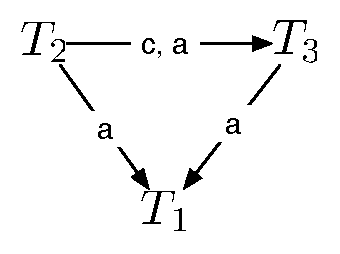
\includegraphics[scale=0.6]{figures/konfliktgraph.pdf}
\caption{Beispiel eines Konfliktgraphen}
\label{default}
\end{center}
\end{figure}


\paragraph{konfliktserialisierbar } ist eine History $H$ 
\begin{itemize}
\item wenn der Konfliktgraph $G_{k}(H)$ azyklisch ist \emph{oder}
\item wenn f\"ur eine serielle History $H_{s}$ gilt: $C(H)$ und $C(H_{s})$ sind konflikt\"aquivalent.
\end{itemize}



\paragraph{sichtserialisierbar}

wenn der zugeh\"orige Konfliktgraph azyklisch ist


\paragraph{Recoverability.} Um Recoverability zu gew\"ahrleisten darf eine Transaktion erst dann committet werden, wenn alle Transaktionen, von denen sie gelesen hat, bereits committet sind. Es muss gelten
$$T_{i} \gets T_{j} \wedge c_{i} \in H \Rightarrow c_{j} <_{H} c_{i}$$
Wenn dies f\"ur eine History $H$ zutrifft schreibt man $H \in RC$.

\paragraph{Cascadelessness / Avoids Cascading Aborts.} Um Cascadelessness zu gew\"ahrleisten und Cascading Aborts zu vermeiden, darf jede Transaktion nur von zuvor committeten Transaktionen lesen. Damit $H \in ACA$ ist muss gelten
$$T_{i} \gets T_{j} \Rightarrow c_{j} < r_{i}[x]$$
Cascadelessness ist eine Einschr\"ankung von Recoverability:
$$ACA \subset RC$$

\paragraph{Strictness.} Um Strictness zu gew\"ahrleisten d\"urfen geschriebene Daten einer noch laufenden Transaktion nicht geschrieben oder gelesen werden. Damit $H \in ST$ ist muss gelten
$$w_{j}[x] < o_{i}[x] (i \neq j) \Rightarrow c_{j} < o_{i}[x] \wedge a_{j} < o_{i}[x]$$
Strictness ist eine Einschr\"ankung von Cascadelessness:
$$ST \subset ACA$$


\paragraph{Korrektheit.}

\begin{table}[htdp]
\begin{center}
\begin{tabular}{lcc}
 & $H \in RC$ & $H \not \in RC$ \\
 \toprule
 $H$ konfliktserialisierbar & ja & nein \\
 $H$ nicht konfliktserialisierbar & & nein \\
\bottomrule
\end{tabular}
\end{center}
\caption{Korrektheit}
\label{default}
\end{table}%



\paragraph{ACID-Eigenschaften}

\begin{description}
\item[Atomicity] 
\end{description}




\subsection{Locking}

\paragraph{Serielle Ausf\"urhung.} 


\section{Logische Anfrageoptimierung}


\paragraph{Grunds\"atze}

\begin{itemize}
\item Selektion so fr\"uh wie m\"oglich
\item Entfernung redundanter Operationen, Idempotenzen und leerer Zwischenrelationen
\item Zusammenfassung gleicher Teilausdr\"ucke
\item Basisoperationen zusammenfassen
\end{itemize}


\end{document}
